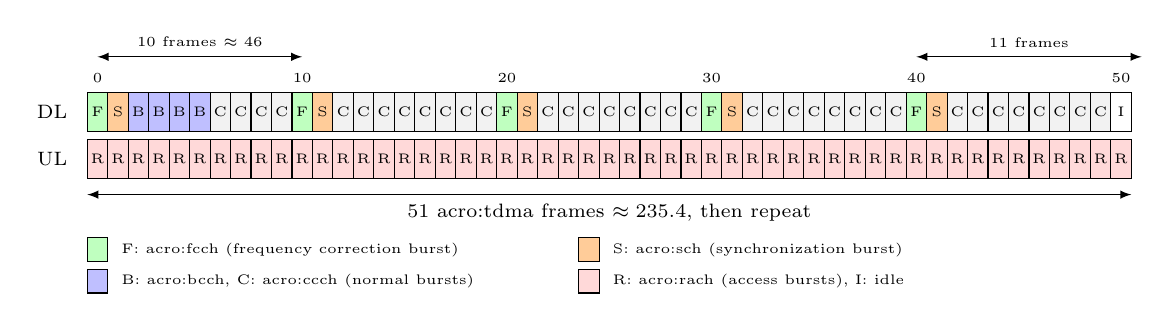
\begin{tikzpicture}[>=latex, x=0.26cm, y=1cm]
    % 51-multiframe on timeslot 0 of the beacon carrier C0 (non-combined configuration)
    \node[anchor=east, font=\scriptsize] at (-0.5,0.85) {DL};
    \foreach \n in {0,...,50} {
        \pgfmathtruncatemacro{\m}{mod(\n,10)}
        \ifnum\n=50 \def\lab{I}\def\col{white}%
        \else\ifnum\m=0 \def\lab{F}\def\col{green!25}%
        \else\ifnum\m=1 \def\lab{S}\def\col{orange!40}%
        \else\ifnum\n<6 \def\lab{B}\def\col{blue!25}%
        \else \def\lab{C}\def\col{gray!10}%
        \fi\fi\fi\fi
        \draw[fill=\col] (\n,0.6) rectangle ++(1,0.5);
        \node[font=\tiny] at ({\n+0.5},0.85) {\lab};
    }

    % Uplink: every frame of timeslot 0 is RACH
    \node[anchor=east, font=\scriptsize] at (-0.5,0.25) {UL};
    \foreach \n in {0,...,50} {
        \draw[fill=red!15] (\n,0) rectangle ++(1,0.5);
        \node[font=\tiny] at ({\n+0.5},0.25) {R};
    }

    % Frame numbers
    \foreach \n in {0,10,20,30,40,50} {
        \node[font=\tiny, anchor=south] at ({\n+0.5},1.1) {\n};
    }

    % Spacing of FCCH bursts
    \draw[<->] (0.5,1.55) -- (10.5,1.55) node[midway, above, font=\tiny] {10 frames $\approx\qty{46}{\milli\second}$};
    \draw[<->] (40.5,1.55) -- (51.5,1.55) node[midway, above, font=\tiny] {11 frames};

    % Total length
    \draw[<->] (0,-0.2) -- (51,-0.2)
        node[midway, below, font=\scriptsize] {51 \gls{acro:tdma} frames $\approx\qty{235.4}{\milli\second}$, then repeat};

    % Legend
    \begin{scope}[shift={(0,-1.05)}, font=\tiny]
        \draw[fill=green!25] (0,0) rectangle ++(1,0.3); \node[anchor=west] at (1.2,0.15) {F: \acrshort{acro:fcch} (frequency correction burst)};
        \draw[fill=orange!40] (24,0) rectangle ++(1,0.3); \node[anchor=west] at (25.2,0.15) {S: \acrshort{acro:sch} (synchronization burst)};
        \draw[fill=blue!25] (0,-0.4) rectangle ++(1,0.3); \node[anchor=west] at (1.2,-0.25) {B: \acrshort{acro:bcch}, C: \acrshort{acro:ccch} (normal bursts)};
        \draw[fill=red!15] (24,-0.4) rectangle ++(1,0.3); \node[anchor=west] at (25.2,-0.25) {R: \acrshort{acro:rach} (access bursts), I: idle};
    \end{scope}
\end{tikzpicture}
